\documentclass[manuscript]{acmart} 

% included in acmart (according to https://www.acm.org/publications/taps/whitelist-of-latex-packages)
% but still necessary somehow
\usepackage{tabularx}

% whitelisted
\usepackage{float}
\usepackage{subfigure}
\usepackage{multirow}
\usepackage[utf8]{inputenc}
\usepackage[nolist]{acronym}

% TabularX column defintions
\newcolumntype{L}[1]{>{\raggedright\let\newline\\\arraybackslash\hspace{0pt}}m{#1}}
\newcolumntype{C}[1]{>{\centering\let\newline\\\arraybackslash\hspace{0pt}}m{#1}}
\newcolumntype{R}[1]{>{\raggedleft\let\newline\\\arraybackslash\hspace{0pt}}m{#1}}

\captionsetup[table]{aboveskip=4pt}
\captionsetup[table]{belowskip=0pt}
\captionsetup{hypcap=false}

\begin{CCSXML}
	<ccs2012>
		<concept>
			<concept_id>10003120.10003121.10003124.10010392</concept_id>
			<concept_desc>Human-centered computing~Mixed / augmented reality</concept_desc>
			<concept_significance>500</concept_significance>
		</concept>
	</ccs2012>
\end{CCSXML}

\ccsdesc[500]{Human-centered computing~Mixed / augmented reality}


\begin{document}
	\begin{acronym}
		\acro{AR}{Augmented Reality}
		\acro{SUS}{System Usability Scale}
	\end{acronym}

	\title{Evaluation of Textual Feedback for Incorrect Usage of an Augmented Reality Application}
	
	\iffalse
	\author{Patrick Harms}
		\affiliation{
			\institution{University of Göttingen}
			\country{Germany}
		}
		\email{EMAIL}

	\author{Julian Lüken}
		\affiliation{
			\institution{University of Göttingen}
			\country{Germany}
		}
		\email{julian.lueken@stud.uni-goettingen.de}
	
	\author{Mehmed Mustafa}
		\affiliation{
			\institution{University of Göttingen}
			\country{Germany}
		}
		\email{EMAIL}

	\author{Jan Schneider}
		\affiliation{
			\institution{University of Göttingen}
			\country{Germany}
		}
		\email{EMAIL}

	\author{Steffen Tunkel}
		\affiliation{
			\institution{University of Göttingen}
			\country{Germany}
		}
		\email{EMAIL}

	\author{Chris Warin}
		\affiliation{
			\institution{University of Göttingen}
			\country{Germany}
		}
		\email{chris.warin@stud.uni-goettingen.de}
	\fi

	% Acronyms go here, refer to them with \ac{shorthand}
	\begin{abstract}
	%	Mobile \ac{AR} applications have gained in importance over the years. Although they provide a variety of uses, they remain mostly unknown by the public, which results in poor understanding of the controls and features from inexperienced users. Improving the usability of mobile \ac{AR} applications is a necessary step to make them more accessible, and finding out how to react to incorrect usage is a part of this process. We conducted a case study to investigate the potential gain in usability provided by feedback messages that assist users when they perform incorrect gestures within mobile \ac{AR} applications. For this purpose, three generic sets of textual feedback (differing in visibility and content) and one control group without feedback were implemented in sets of two \ac{AR} applications, each application displaying a different \ac{AR} prototype (a microwave or a toaster). The applications detected pinch-zoom and two-finger rotation gestures as incorrect input. In total, 40 participants have been addressed to execute a predefined set of tasks and their incorrect inputs when using the mobile \ac{AR} have been evaluated. Several analyses have been carried out: the mean values of the control group only differ significantly from the group receiving the most supportive feedback regarding the time needed to complete the set of tasks and the number of attempts of incorrect two-finger rotations. An overall positive correlation could also be found between both variables. Finally, the SUS score calculated from an adapted SUS questionnaire descriptively showed that the presence of feedback in general improved the usability, although there was no clear difference in score between the case study groups. When given appropriate feedback, most people still performed incorrect gestures, but quickly recovered from mistakes and were much less likely to do them again. However, more data is needed to further evaluate the feedback given for the pinch-zoom gesture. Further research should be conducted to evaluate the impact of feedback types other than textual as well as the separate impact of visibility and content on mobile \ac{AR} usability. 
	Although mobile Augmented Reality (AR) applications gained in importance over time, inexperienced users still handle them poorly and use inappropriate gestures, e.g., pinch-zoom. To address this, we evaluated the impact of feedback messages to improve the learnability of AR. We implemented two AR applications and three generic sets of textual feedback, with different visibility and content, and compared them with a control group without feedback. Pinch-zoom and two-finger rotation gestures were detected as inappropriate inputs. We analysed the data of 40 test users of our AR applications. Our most supportive feedback achieved a reduction of the time needed to complete a set of tasks and of the number of incorrect two-finger rotations. The results of an SUS questionnaire descriptively showed that the presence of feedback improves the user-perceived usability. When given appropriate feedback, most people recovered quickly from mistakes and were less likely to redo them.
	\end{abstract}
	\keywords{Augmented Reality, Usability, Feedback, Mobile, Case Study}
	\maketitle
	\pagebreak
	\section{Introduction}\label{sec:introduction}
		In recent years, the number of available mobile \ac{AR} applications for smartphones has increased~\citep{Tractica2017}. Although mobile \ac{AR} technology is no novelty, it was not widely available for public until most smartphones became capable of running \ac{AR} applications. Since most users are newly discovering \ac{AR} technology, they do not know how to use its features yet. Instead, they use unsupported gestures as inputs, which leads to frustration. Our main motivation for conducting this research is the lack of good feedback in case of incorrect usage, which could help a lot of users to avoid repeating common mistakes while using \ac{AR} applications for smartphones. Providing good feedback could also help and teach users to control such \ac{AR} applications without the need of a separate introduction.

		Our research goal is to provide appropriate feedback to unsupported gestures and decide what type of textual feedback is the best. Our work is guided by the research question: ``How can feedback on incorrect gestures in mobile AR improve its usage?''. Therefore, we defined 3 different types of feedback. To evaluate which variant works best, we conducted a usability case study. In this study, we asked 40 test participants to interact with virtual prototypes of technical devices visualized in mobile \ac{AR}. The participants were subdivided into four groups, where one group got no feedback at all and the three other ones were provided with one of our proposed feedback approaches. Our results show that one of our approaches improves the mobile \ac{AR} usage.

		The organization of the paper is as follows. Section~\ref{sec:foundations} gives information about usability in general and the mobile \ac{AR} environment that we use in our case study. In Section~\ref{sec:relatedwork} we discuss similar work on \ac{AR} and feedback done in the past. Section~\ref{sec:approach} gives a detailed illustration of the three feedback types we present to users. In Section~\ref{sec:casestudy}, we describe the setup of our case study, as well as our results and the discussion thereof. Finally, we summarize our result and give an outlook on future work in Section~\ref{sec:summary}.

	\pagestyle{myheadings}
	\section{Foundations}\label{sec:foundations}
		% * What is AR?
		The main goal of our work is to find suitable user feedback for mobile \ac{AR} applications. In this section, we first clarify our notion of mobile \ac{AR} and describe the technologies we use. The generic term \ac{AR} itself describes a variety of technologies that place 3D virtual objects into a 3D real environment in real time. This can be achieved by a handheld device like a mobile phone (mobile \ac{AR}) or using wearable goggles like the Microsoft HoloLens. In this paper we focus on \ac{AR} for mobile phones, where recorded imagery of the phone is being augmented and shown to the user to display a mix of virtual objects and the real world at runtime. Examples for this are shown in Figure~\ref{fig:feedbackonphone}. Parts (a) and (b) visualize a virtual toaster with toastable bread on real world tables. Part (c) visualizes a virtual microwave and a slize of pizza on a virtual plate.
		\begin{figure}[H]
			\centering
			\subfigure[]{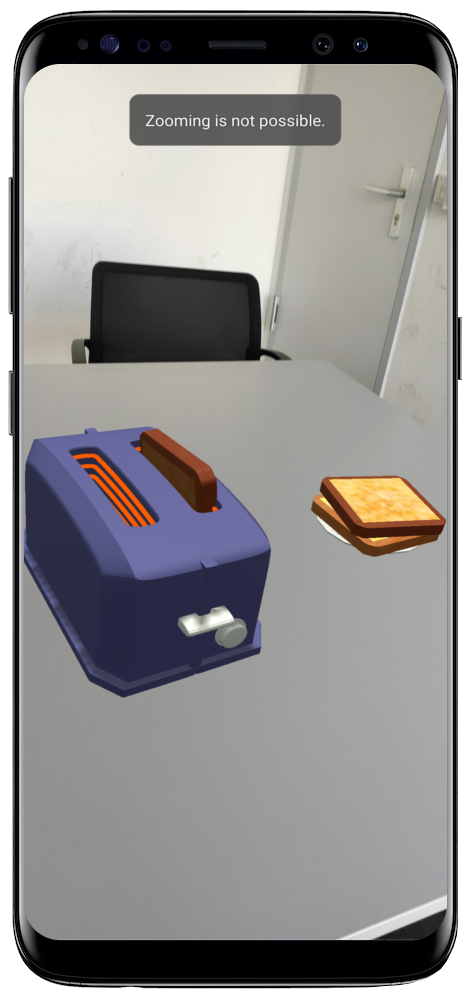
\includegraphics[width=.28\textwidth]{img/phone/phonepz1.png}}
			\subfigure[]{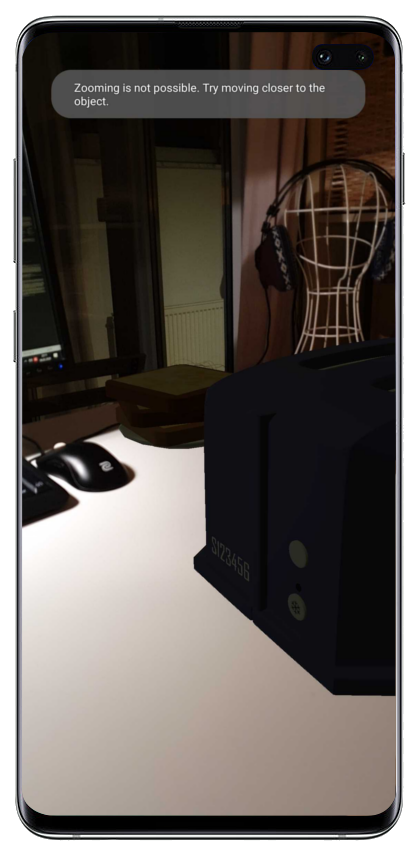
\includegraphics[width=.28\textwidth]{img/phone/phonepz2.png}}
			\subfigure[]{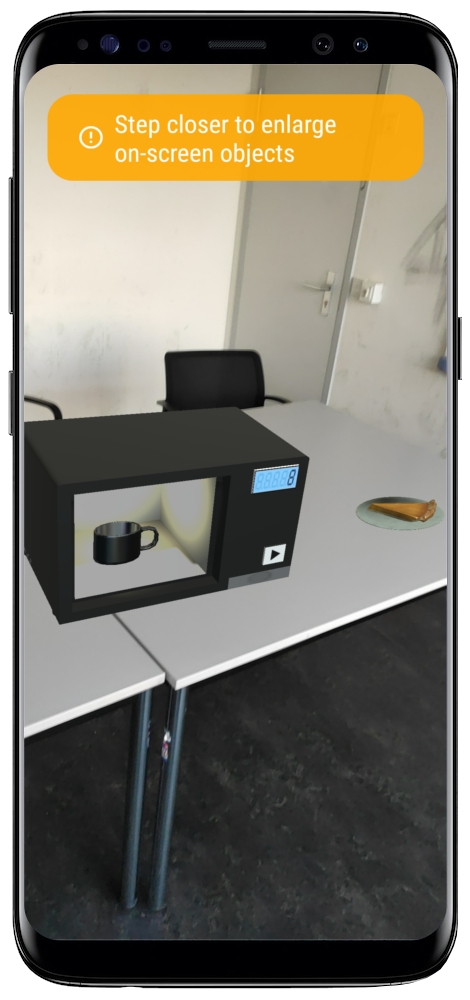
\includegraphics[width=.28\textwidth]{img/phone/phonepz3.png}}
			\caption{Three screenshots of an app made with the Vivian framework.}
			\label{fig:feedbackonphone}
			\Description{Three screenshots of an app made with the Vivian framework}{}
		\end{figure}
		% * Which frameworks/technologies were used?
		%     * Brief info about Vivian (which relies on state machines)
		%         * What gestures are "correct"? (vivian relies on 1 finger shit and moving environment)
		The tasks that we ask our users to execute in our case study consist of different interactions with virtual prototypes of technical devices as shown in Figure~\ref{fig:feedbackonphone}. A virtual prototype is a \textit{``\textnormal{[…]} computer simulation of a physical product that can be presented, analyzed, and tested from concerned product life-cycle aspects such as design/engineering, manufacturing, service, and recycling as if on a real physical model.''}~\cite{Wang2002}. In our study those virtual objects are prototypes of technical devices like a microwave or a toaster. For the implementation of those prototypes we used the Vivian framework. It is an extension for the game engine Unity3D~\cite{Unity}, that can be used to create mobile \ac{AR} implementations of virtual prototypes using a 3D model and finite-state machines. In a mobile app made with the Vivian framework, all user inputs rely on one finger gestures on the touch screen. Examples for virtual prototypes visualized by Vivian in mobile AR are shown in Figure~\ref{fig:feedbackonphone}. Users can interact with the different 3D models on the screen. Buttons can be pressed by simply tapping the screen where the respective button is displayed. Knobs and levers can be moved by putting a finger on the screen where the knob or lever is displayed, moving the finger on the screen until finding the desired position, and removing the finger from the screen afterwards. We refer to this gesture as \emph{drag-and-drop}. The Vivian framework makes a clear distinction between movable and non-movable objects in a scene. The slice of bread in part (a) of Figure~\ref{fig:feedbackonphone} example is movable, whereas the toaster itself cannot be moved. Movable objects can be moved in the same fashion as a lever. To cover greater distances, one can move the device itself while dragging the object. Rotation similarly requires the user to hold their finger on the object and rotate the device until they find the desired orientation.

		The limit of one-finger-interactions exists due to the peculiarity of mobile \ac{AR} environments. Two-finger-interactions (like a pinch-zoom or a two-finger-rotation) would contradict the intended design of such an environment. If users want to take a closer look at a virtual object, they would need to step closer to it instead of performing a pinch-zoom. Instead of a two finger rotation, users should interact more realistically, by grabbing an object using the mobile phone's screen and rotating it using the mobile phone's rotation.

		To evaluate different types of feedback, we decided to use usability testing as a tool to quantify the corresponding results. According to Nielsen, \textit{``usability is a quality attribute that assesses how easy user interfaces are to use. The word "usability" also refers to methods for improving ease-of-use during the design process.''}~\cite{Nielsen2012}. Usability testing refers to an \textit{``observational methodology to uncover problems and opportunities in designs''} with the goal to identify problems in the design of the product or service. It also helps to uncover opportunities to improve and to learn about the target user's behavior and preferences~\cite{Moran2019}.

		In addition to observing users while interacting with a product or service, an established method is the usage of questionnaires. Those can help to find out about the users' attitude towards the product as well as the main issues they experienced. A well-known questionnnaire is the \acf{SUS}~\cite{SUS2019}. It is a single choice questionnaire which consists of ten items with five response options, ranging from 0 (\emph{strongly disagree}), to 4 (\emph{strongly agree}). Odd numbered questions are phrased positively towards the system in question, whereas even numbered questions are phrased negatively. For the evaluation, responses to the negative questions are subtracted from 5. The responses are then added together and multiplied by 2.5, yielding the so called SUS score, which lies between 0 and 100, where 100 means good usability. A mean SUS score of 68 stands for average usability.

	\section{Related Work}\label{sec:relatedwork}
		The topic of error handling in \ac{AR}-applications has not been broadly studied yet. There are several guidelines on how to handle wrong user input. Microsoft states in its design guidelines, that error messages should alert users of an already occurred problem~\cite{Microsoft2018}. Another point they make is that the message should be suppressed if it does not make the users change their behavior or perform an action~\cite{Microsoft2018}. In addition to that, Nielsen's \textit{Error Message Guidelines} demand error messages to be phrased politely. This is to avoid the impression that the user did something stupid or inherently wrong. It is also important that the messages are precise descriptions of exact problems, offering constructive advice on how to fix the problem~\cite{Nielsen2001}.

		\citeauthor{Poupyrev2002} discuss two approaches of how user help might be implemented in \ac{AR} environments. They offered  an icon which the users might activate themselves when they seek advice for a given task. The other feature was an automated help message that pops up when the user moves an object associated to a certain task closer to his face and tilts it. They state, that \textit{"\textnormal{[t]}his approach is more suitable for AR interfaces than traditional desktop help systems, which either distract users with a constant barrage of help messages or interrupt their work by making them search explicitly for help."}~\cite{Poupyrev2002}.
		
		Our work ties in with these principles by seeking to find useful feedback after the occurrence of incorrect user input. The main focus is to give users helpful advice when interacting with mobile AR in an AR-contradicting manner.

	\section{Approach}\label{sec:approach}
		The goal of our work is to provide users of mobile \ac{AR} with feedback in case of unsupported interactions. For this, we developed three types of feedback messages. Each differs in content, color, and size (see Figure~\ref{fig:feedbackonphone}). In this section, we will first describe the most common user input gestures made on the touch screen which do not work in mobile \ac{AR}. Then, we present the exact content of our feedback messages and the conditions under which they appear.

		\subsection{Inappropriate Gestures in Mobile AR}\label{ssec:incorrectinput}
		\ac{AR} applications have a certain concept for interaction. This covers that virtual objects have fixed poses in the real world. To see more details of an object, users can either move it closer to themselves or they move closer to the object. For rotating objects, users first grab the object and then turn it into the intended direction.
		Depending on the mobile \ac{AR} application, these concepts are implemented differently. The implementation in the example of the Vivian framework is described in Section~\ref{sec:foundations}. The interactions that do typically not work with mobile \ac{AR} as they do with traditional mobile apps are \emph{pinch-zoom} and \emph{two-finger rotation}.

		The pinch-zoom is a gesture in which two fingers are placed on the touch screen and moved apart in opposite directions. The two-finger rotation is a gesture in which two fingers are placed on the touch screen and are together moved clockwise or counterclockwise around the center of the positions of the fingers. A two-finger rotation can also be executed by only moving one of the fingers clockwise or counterclockwise around the other finger.

		In common mobile apps, pinch-zoom is used to enlarge objects. In mobile \ac{AR}, this gesture may also be applicable, but only if users intend to scale objects. But more often, they want to see more details of the virtual objects for which the correct gesture would be to reduce the distance between the object and themselves, e.g. by stepping closer. The two-finger rotation in common mobile apps always has a clear rotation axis being the screen normal. In mobile \ac{AR}, it may not be the screen normal, but e.g. one of the axes of the coordinate system. Despite of these uncertainties, our research shows that users try to use known gestures for smartphone interaction. Therefore, they also typically try pinch-zoom and two finger rotation in mobile \ac{AR}. Our feedback messages are shown in case one of these gestures is tried by the users.

		\subsection{Feedback Message Types}\label{ssec:feedbackmsgs}
		We developed three types of feedback messages occuring in case the users of mobile AR use either the pinch-zoom or the two-finger-rotation gestures. The content of the first feedback message type is a \emph{critique}. If the user inputs a gesture that we consider incorrect, the app outputs a message that said input is not possible. For example, if a user tried pinch-zooming, they would receive a message saying: ``Zooming is not possible'' (see Figure~\ref{fig:feedbackonphone} (a)). The content of the second feedback message type is \emph{critique} and \emph{support}. We refer to this feedback type as \emph{combined} in the course of this paper. The user is provided with a message stating that above mentioned input is not possible and the app gives a hint on what they should try instead. In the scope of the previous example, such a message would say: ``Zooming is not possible. Try moving around the object'' (see Figure~\ref{fig:feedbackonphone} (b)). In the first two types, the messages have the same size and color scheme. The third type is a more concise \emph{support}. For our previous example the exact message is saying: ``Step closer to enlarge on-screen objects''. It also differs in color scheme and size (see Figure~\ref{fig:feedbackonphone} (c)). Each feedback message of every type is displayed for 5 seconds.

		The contents of each message can be found in Table~\ref{tab:feedback}. The description column holds the names we assigned to the three different feedback types. In the gesture and response columns you can find the corresponding inputs and outputs respectively. If for example a user tries a two-finger rotation in the critique implementation, the app would display a message saying ``Rotating the object is not possible''.

		\begin{center}
		\begin{table}
			\captionof{table}{The responses for each input in each implementation.}
			\begin{tabular}{|C{.05\textwidth}|L{.15\textwidth}|L{.23\textwidth}|L{.45\textwidth}|} \hline
										& \textbf{Description}												& \textbf{Gesture (input)} 					& \textbf{Response (output)} 											\\ \hline
				\multirow{2}{*}{\#1}	& \multirow{2}{*}{\parbox{.15\textwidth}{critique}}					& two-finger rotation						& Rotating the object is not possible.									\\ \cline{3-4}
										& 																	& pinch-zoom								& Zooming is not possible. 												\\ \hline
				\multirow{2}{*}{\#2}	& \multirow{2}{*}{\parbox{.15\textwidth}{combined}}					& two-finger rotation						& Rotating the object is not possible. Try moving around the object.	\\ \cline{3-4}
										& 																	& pinch-zoom								& Zooming is not possible. Try moving closer to the object.				\\ \hline
				\multirow{3}{*}{\#3}	& \multirow{3}{*}{\parbox{.15\textwidth}{support}}					& two-finger rotation (movable object)		& Hold the object and move the phone to rotate							\\ \cline{3-4}
										& 																	& two-finger rotation (elsewhere)			& Move around the objects												\\ \cline{3-4}
										&																	& pinch-zoom 								& Step closer to enlarge on-screen objects								\\ \hline
			\end{tabular}
			\label{tab:feedback}
		\end{table}
		\end{center}

		Table~\ref{tab:feedback} also shows that in the support implementation we made the distinction between two-finger rotations on movable objects and elsewhere. If the aforementioned center point of the two-finger rotation is placed on a movable object (see Section~\ref{ssec:incorrectinput}), the app displays the message ``hold the object and move the phone to rotate''. If the two-finger rotation is executed elsewhere, the ``move around the objects'' message is displayed instead. We recognize user input using a software library called TouchKit~\cite{TouchKit}. TouchKit provides an easy way to detect gestures such as our two-finger rotations and pinch-zooms.

	\section{Case Study}\label{sec:casestudy}
		To evaluate the quality of our feedback implementations we conducted a case study. In this case study, we asked participants to interact with a mobile AR. Our goal was to trigger pinch-zoom and two-finger-rotation interactions and to see which feedback message type helped the participants best to find the correct interaction. In this section we describe in detail what each participant in the case study had to do and what data we collected. Then we provide our results and discuss their meaning.
		
		\subsection{Setup of the Case Study}\label{ssec:setup}
			In order to evaluate, which feedback message type works best, we created two different virtual prototypes with the Vivian framework (see Section~\ref{sec:foundations}). Both of them are simplified kitchen devices: a toaster and a microwave (as seen in Figure~\ref{fig:feedbackonphone}).

			The microwave's functionality is limited to heating an object inside it with constant power. Figure~\ref{fig:feedbackonphone} (c) shows this prototype in a mobile \ac{AR} application. It has one button to add 10 seconds to the heating duration and another one below to open the door. The door can be closed by moving it. The status of the microwave is visually indicated by a small display showing the remaining heating time or ``ready'' in idle mode. Furthermore, there is a light inside the device, which turns on when it is heating or when the door is opened. A serial number is printed on the back of the device. The prototype scene is completed by two additional objects, being a cup that is already in the microwave when the application launches and a piece of cake on a plate next to it. These objects are movable by the user.

			The toaster can toast one or two pieces of bread at a time. Figure~\ref{fig:feedbackonphone} (a) shows the front of the prototype in a mobile \ac{AR} application and Figure~\ref{fig:feedbackonphone} (b) its back. The toasting can be started by pulling down a lever at the front and stopped by pushing it up again or by pressing the stop button, which is on the back. Otherwise, the toasting stops automatically after a time which is defined by the position of a rotatable knob at the front. The time mode is divided into low, medium and high duration. Further functionality is provided by the unfreezing mode, which can be activated using the snowflake button on the back. The activation of the unfreezing mode results in a longer toasting duration and is indicated by a light above the button. The toasting process itself is displayed by the glowing of the heating elements, which is visible in Figure~\ref{fig:feedbackonphone} (a). The toaster prototype also has a serial number on its back. The prototype scene is completed by a stack of 3 pieces of bread lying next to it. 
			
			Based on these functionalities we designed three tasks per virtual prototype, which are shown in Table~\ref{tab:tasks}. The tasks are increasing in complexity. An example of this increase is that in task 2 of the microwave we ask to heat the cup, which is already in the microwave, for any amount of time. Therefore, only the start button has to be pressed once to fulfill this task. Afterwards, in task 3, we ask to replace the cup with the pie and heat for a specific amount of time. This task contains more necessary steps: opening the door, moving the cup out, moving the pie in, closing the door, pressing the start button multiple times and finally pressing the stop button after the desired amount of time. 

			\begin{center}
				\begin{table}[H]
					\captionof{table}{The tasks for the different prototypes.}
					\begin{tabular}{|C{.05\textwidth}|L{.41\textwidth}|L{.41\textwidth}|}
						\hline \textbf{\#} & \textbf{Microwave} & \textbf{Toaster} \\
						\hline 1 & Read serial number of the microwave & Read serial number of the toaster \\
						\hline 2 & Heat up the cup & Toast the bread \\
						\hline 3 & Remove the cup, put the pie in, set the timer to 20 seconds and remove the plate at 5 seconds & Toast the bread on high heat and put the toaster in unfreezing mode \\
						\hline
					\end{tabular}
					\label{tab:tasks}
				\end{table}		
			\end{center}

			For the case study, we divided the participants into four groups. Each of these groups tested one version of the app on a mobile phone. The versions differed in the feedback message types given (see \emph{\nameref{sec:approach}}). We gave no feedback at all to the participants in group 0, which is our control group. Participants in group 1 got the \emph{critique} feedback. In group 2 they got the \emph{combined} feedback version and in group 3 they got the  \emph{supportive} feedback (see Table~\ref{tab:feedback}). Each participant was asked to fulfill the tasks for each prototype in the order provided in Table~\ref{tab:tasks}. One half of the participants were asked to do the tasks of the toaster first, while the other half did the tasks for the microwave first. This divide was equally for all groups.

			Before the start of the test, we gave every participant a short introduction. This introduction contains information about the mobile \ac{AR} technology and reasons behind usability testing to prepare the participants and create a similar level of expectation. It deliberately does not contain information about how to use the application or the scope of the case study. This is important so the participants are not biased about wrong usage and the feedback they would get. During the test, we used screen recordings to measure each participants' use of the application. These enabled us to acquire completion times for the different tasks and count the number of incorrect usages. We used a notepad to register further observations.

			Following the test of the application, the participants were asked to fill in a questionnaire. This questionnaire consists of 3 parts. First we asked participants if they had used \ac{AR} applications before. The second part is an \ac{SUS} (see Section~\ref{sec:foundations}) about the usability of the \ac{AR} application. In the \ac{SUS}, the word ``system'' was replaced by ``AR app''. The first question was changed from ``I think that I would like to use this system frequently'' to ``I can think of a reasonable scope of application for this AR app in which I would use it frequently''. The second question was changed from "I found the system unnecessarily complex'' to ``I found the controls of the AR app unnecessarily complex''. The last question was changed from ``I needed to learn a lot of things before I could get going with this system'' to ``I found it hard to recover from mistakes in the AR app''. The third part is an open question directly aimed at the feedback provided by the application, namely: \emph{``If you have any suggestions on what kind of feedback from the app you would find better, please let us know''}.

		\subsection{Results of the Case Study}\label{ssec:results}
			We conducted the case study with 10 participants per feedback group. This leads to 40 people participating in the case study in total. 21 of the 40 participants said they had prior experience with \ac{AR} applications. The group with the highest prior knowledge was the control group with 7 of 10 participants. The groups for the \emph{critique} feedback and the \emph{combined} feedback both had 6 participants with prior knowledge, while the group with the \emph{support} feedback had just 2 participants, who said they had prior knowledge.

			In our approach, we consider especially two gestures as incorrect usage: the pinch-zoom and the two-finger rotation (see Section~\ref{sec:approach}). With the setup of our case study, the two-finger rotation appeared more often than the pinch-zoom gesture. Figure~\ref{fig:tfr_v_pz} shows the appearances of two-finger rotations and pinch-zooms for all tasks given to the participants in the case study. In total over all participants and all tasks, two-finger rotations appeared 225 times, while pinch-zoom appeared 51 times. The task where users used these two gestures the most was the second task for the toaster. As shown in Figure~\ref{fig:tfr_v_pz} (a), 91\% of the overall two-finger rotations occurred in that task. Also the majority of pinch-zoom gestures occurred there.

			\begin{figure}[H]
				\centering
				\subfigure[]{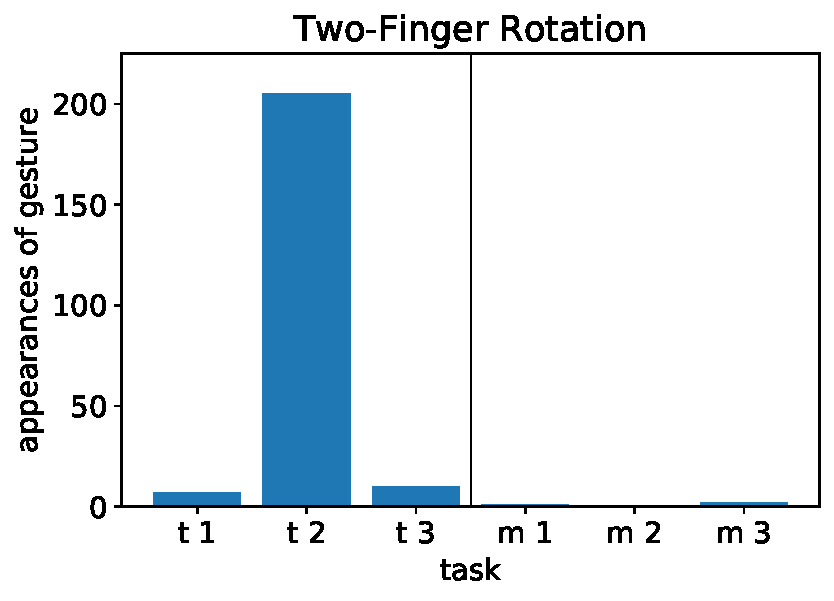
\includegraphics[width=.49\textwidth]{img/plot/plot_tfr.pdf}}
				\subfigure[]{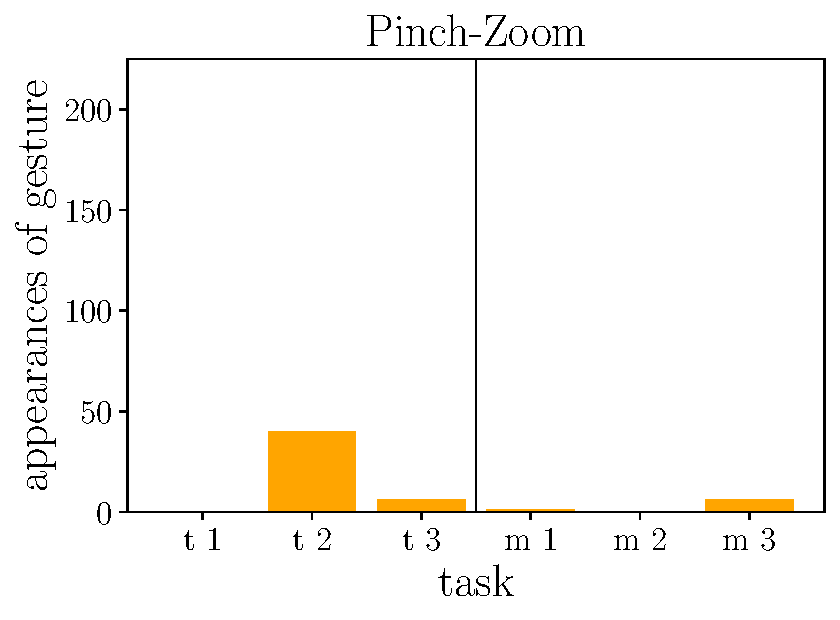
\includegraphics[width=.49\textwidth]{img/plot/plot_pz.pdf}}
				\caption{Appearances of the two-finger rotation gesture and the pinch-zoom gesture per task of the case study.}
				\label{fig:tfr_v_pz}
				\Description{Appearances of the two-finger rotation gesture and the pinch-zoom gesture per task of the case study.}{}
			\end{figure}

			To evaluate the effectiveness of the different feedback types, we compared the users' behavior within the different tasks. We exemplify this comparison for task 2 for the toaster. Figure~\ref{fig:t2_metrics} shows box plots for the two most important measures. The diagram in Figure~\ref{fig:t2_metrics} (a) gives the time participants needed to fulfill the task by their case study group. The median is given by the horizontal line inside the box. The box itself gives the 25 percentile on its lower bound and the 75 percentile on its upper bound. The whiskers are defined by the last data points which are within the range of 1.5 times the interquartile range. For clarification, the data points are printed semi-transparent over the box plot. Figure~\ref{fig:t2_metrics} (b) is similar: it shows the two-finger rotation attempts per user for the different case study groups. In total, 4 of the 40 participants didn't try any two-finger rotations in this task.

			\begin{figure}[H]
				\centering
				\subfigure[]{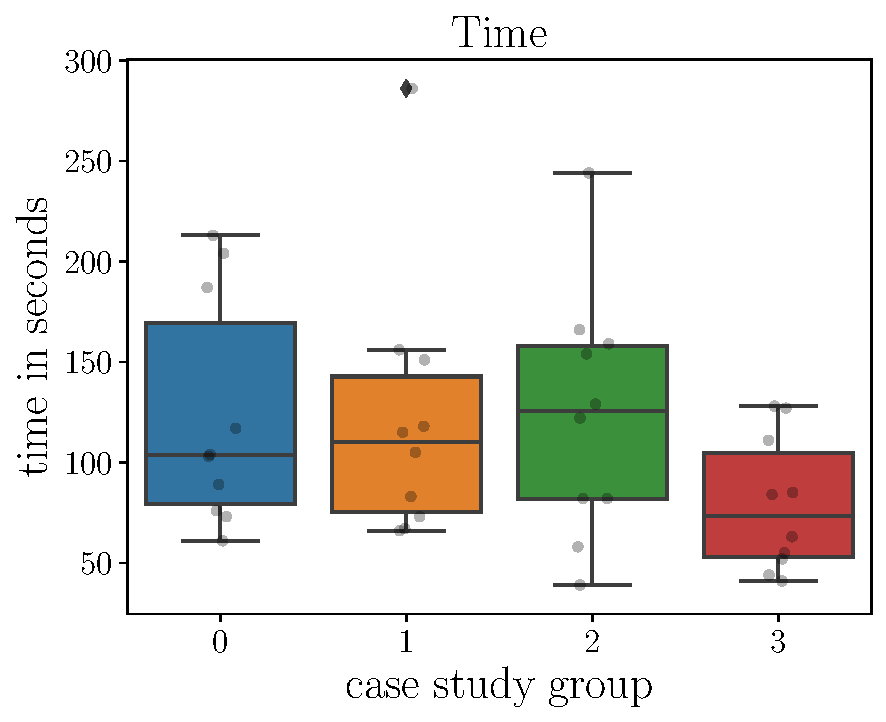
\includegraphics[width=.49\textwidth]{img/plot/plot_bplot_time.pdf}}
				\subfigure[]{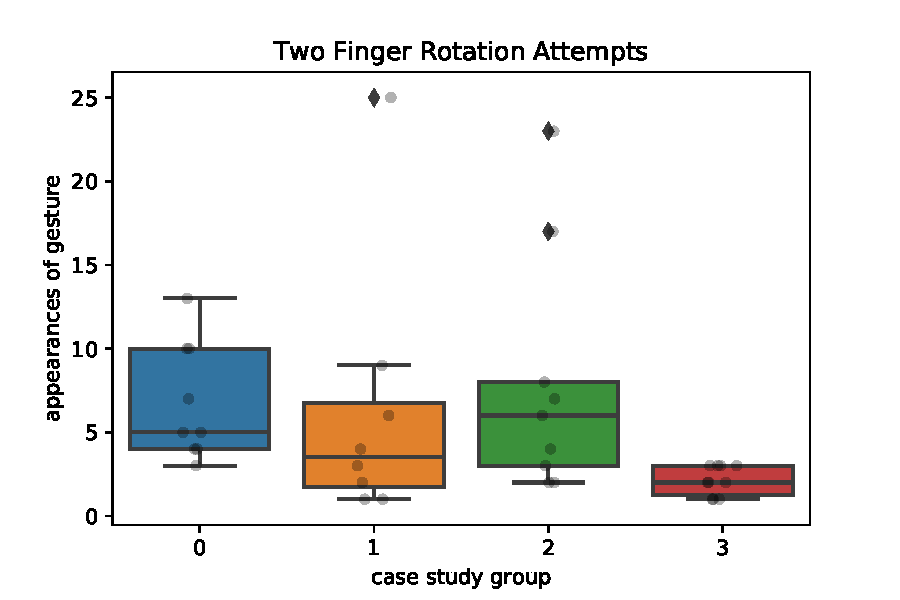
\includegraphics[width=.49\textwidth]{img/plot/plot_bplot_tfr.pdf}}
				\caption{Evaluation of the time (a) and the two-finger rotation attempts (b) needed for the second task for the toaster prototype.}
				\label{fig:t2_metrics}
				\Description{Evaluation of the time (a) and the two-finger rotation attempts (b) needed for the second task for the toaster prototype.}{}
			\end{figure}

			To check whether our result is statistically significant, we used the \emph{Kruskal-Wallis one-way analysis of variance} to compare the number of two-finger rotation attempts in the different feedback groups to the control group. The \emph{Kruskal-Wallis test} does not assume normal distribution of measurements among the groups. The test takes multiple samples as input and returns the significance $p$ and a statistic $H$ that is related to the effect size $\eta^2 = \frac{H-k+1}{n-k}$, where $k$ is the number of groups and $n$ is the combined size of the input samples~\cite{Tomczak2014}. Generally, we consider an effect with $p < \alpha_0 = 0.05$ as statistically significant and $\eta^2 \in [0.01,0.06)$ as small, $\eta^2 \in [0.06,0.14)$ as moderate and $\eta^2 \geq 0.14$ as large. Since we calculated one test for each feedback type, we applied Bonferroni correction to $\alpha_0$, yielding $\alpha_1 = \frac{\alpha_0}{3} \approx 0.0167$. The number of two-finger rotations in the second toaster task with \emph{critique} feedback has shown no significant effect ($H = 1.9735$ with $n_\text{dof} = 1$, $p = 0.1601$). The number of two-finger rotations in the second toaster task with \emph{combined} feedback has shown no significant effect ($H = 0.0705$ with $n_\text{dof} = 1$, $p = 0.0037$). The number of two-finger rotations in the second toaster task with \emph{supportive} feedback is significantly lower than control ($H = 8.4483$ with $n_\text{dof} = 1$, $\eta^2 = 0.4138$, $p = 0.0037$). The users' completion times in this task support this finding (see Figure~\ref{fig:t2_metrics} (a)).

 			In the other tasks, we found that users were not often using pinch zooms or two-finger rotations (as Figure~\ref{fig:tfr_v_pz} suggests), such that the median of incorrect gestures for almost every group in almost every task is 0. That is why no further two groups were comparable by the number of wrong gestures. Therefore, we did not perform statistical testing with the remaining data.

 			\iffalse
			\begin{center}
			\begin{table}
				\captionof{table}{$p$-values of statistical tests for the time needed to fulfill the 2nd task for the toaster prototype and the two-finger rotation attempts in that task.}
				\begin{tabular}{|L{.22\textwidth}|L{.22\textwidth}|C{.22\textwidth}|C{.22\textwidth}|} \hline
					\textbf{statistical test}		& \textbf{implementation}	& \textbf{p-values: time} 		& \textbf{p-values: two-finger rotation} 											\\ \hline
					\multirow{3}{*}{Shapiro-Wilk}	& critique					& 0.972							& 0.001								\\ \cline{2-4}
													& combined					& 0.029							& 0.420 								\\ \cline{2-4}
													& support					& 0.507							& 0.971								\\ \hline
					\multirow{3}{*}{Welch t-test}	& critique					& 0.980							& -								\\ \cline{2-4}
													& combined					& - 							& 0.681									\\ \cline{2-4}
													& support					& 0.054							& 0.010 									\\ \hline
				\end{tabular}
				\label{tab:pvalues}
			\end{table}
			\end{center}
			\fi

			In addition, we evaluated the relationship between our two metrics for the task. The correlation coefficient between the time and the attempts of two-finger rotation is 0.43, which indicates a moderate positive relationship between the metrics. Figure~\ref{fig:scatter} visualizes the relationship between the time needed for the task and the number of two-finger rotation tries. The color of a data point is set by the implementation used by this participant. One can observe that the participants with implementation 3, which are shown by the red data points, are all clustered with a low time and a low amount of two-finger rotations, while all other groups are more randomly spread.

			\begin{figure}[H]
				\centering
				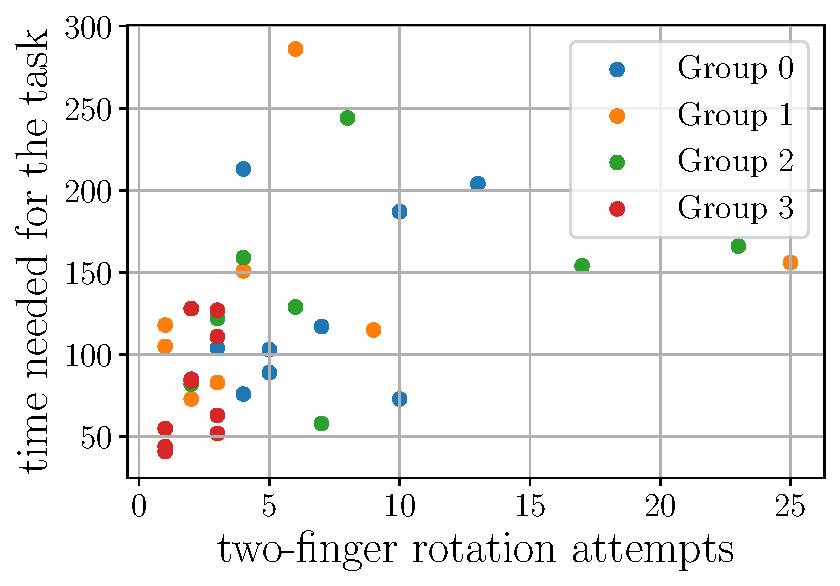
\includegraphics[width=.49\textwidth]{img/plot/plot_scatter.pdf}
				\caption{Time needed to fulfill the 2nd task for the toaster prototype depending on the count of two-finger rotation attempts.}
				\label{fig:scatter}
				\Description{Time needed to fulfill the 2nd task for the toaster prototype depending on the count of two-finger rotation attempts.}{}
			\end{figure}

			For the evaluation of the questionnaire, we calculated the \ac{SUS} scores for every participant. Figure~\ref{fig:sus} shows the mean score for each case study group. The horizontal red line is at a score of 68, which in terms of \ac{SUS} stands for average usability. The figure shows that the mean \ac{SUS} result of participants in case study group 3 with the support implementation is slightly higher than the mean of case study groups 2 and 3. The mean \ac{SUS} score of the control group is the lowest. Comparing group 3 to the control group yields no statistically significant effect ($H = 1.2151$ with $n_\text{dof} = 1$, $p = 0.2703$).

			\begin{figure}[H]
				\centering
				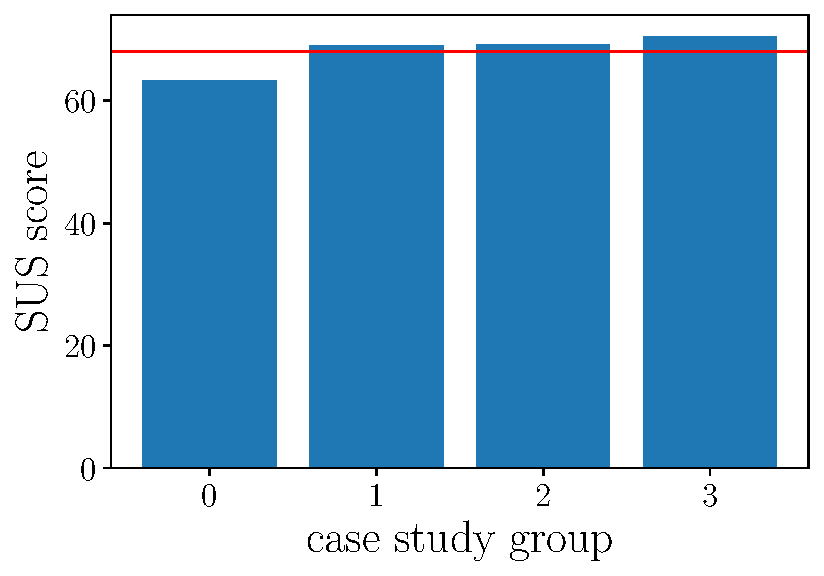
\includegraphics[width=.49\textwidth]{img/plot/plot_sus.pdf}
				\caption{SUS score by the case study groups.}
				\label{fig:sus}
				\Description{SUS score by the case study groups.}{}
			\end{figure}

			24 of the 40 participants answered the open question. We categorize the answers with four different labels, divided by the topic the answer is about. These are \emph{app feedback}, \emph{app controls}, \emph{prototype design} and \emph{other}. Answers in the \emph{app feedback} category are directed to the provided feedback messages or other desired feedback. Answers in the \emph{app controls} category are about struggles with or improvement ideas for the applications controls. The \emph{prototype} category is related to the prototype design and its usability, for example button sizes. The last category, \emph{other}, is summing up single appearing answers whose scope is not relevant for this research. The appearances of the different types of answers are listed in Figure~\ref{fig:tags}. In case an answer fits to multiple labels, we count it for all the fitting categories.

			\begin{figure}[H]
				\centering
				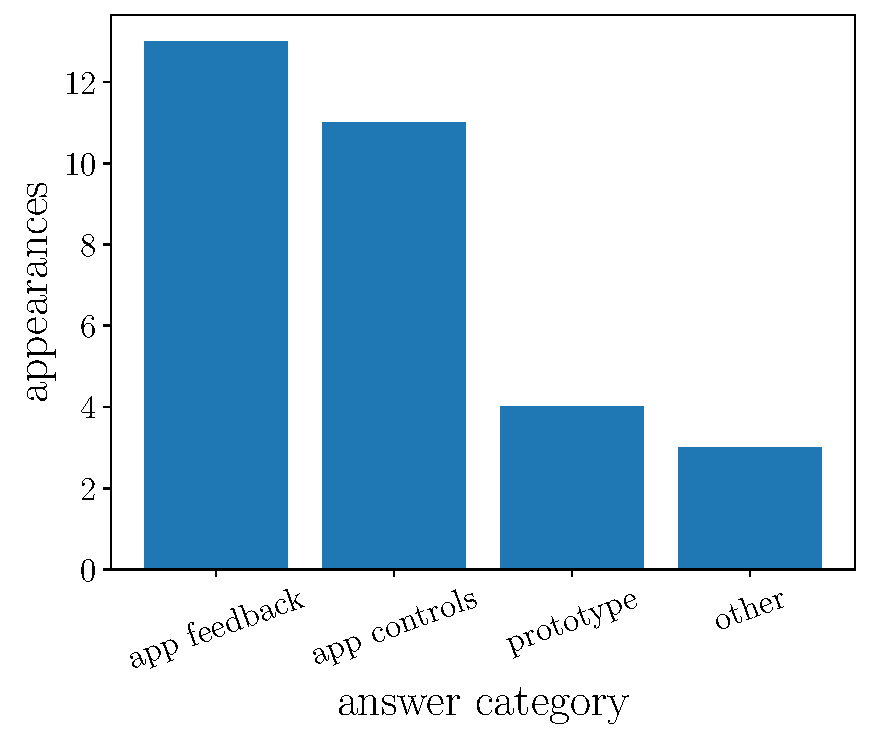
\includegraphics[width=.49\textwidth]{img/plot/plot_tags.pdf}
				\caption{Categorized open question answers.}
				\label{fig:tags}
				\Description{Categorized open question answers.}{}
			\end{figure}
			
			For a deeper evaluation of the answers we split them by the case study groups (see Figure~\ref{fig:tags_imp}). 
			Most of the answers related to \emph{app feedback} came from participants in the control group. All of these answers were asking for any kind of help. Two of them directly asked for text messages providing help. Also the ideas of a help button or an introduction, which explains the controls were mentioned. Participants in the other groups also mentioned additional help implementation methods, like vibration feedback or help for the specific task from the application. Answers directed to our feedback message implementations were that they could be hidden by the fingers, when the user turns the phone and one participant with the \emph{combined} feedback mentioned that the message should be visible for a longer duration.

			The other big category of the participants' answers is \emph{app control} related. They have in common that the rotation of the piece of bread in the second task for the toaster prototype was not easy to achieve for them. Also some were mentioning that the two-finger rotation could be the more intuitive option.

			\begin{figure}[H]
				\centering
				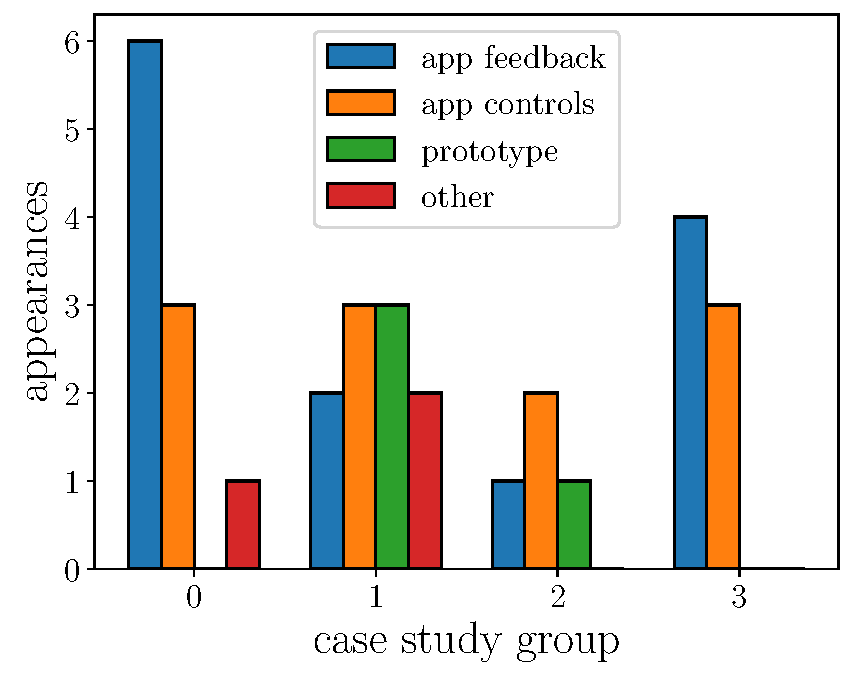
\includegraphics[width=.49\textwidth]{img/plot/plot_tags_implementations.pdf}
				\caption{Appearances of answer categories by the participants case study groups.}
				\label{fig:tags_imp}
				\Description{Appearances of answer categories by the participants case study groups.}{}
			\end{figure}

		\subsection{Discussion of the Case Study Results}\label{ssec:discussion}
			With the given setup of our case study, the two-finger rotation gesture appeared more often than the pinch-zoom gesture (see Figure~\ref{fig:tfr_v_pz}). We assume users attempt to use the pinch-zoom gesture when an object on the screen is too small to see or use. Given this, the participants were not tempted to pinch-zoom, because they started right in front of the objects. Also, for simplicity's sake, the prototypes were not created with unnecessarily small controls, which means all of them were well visible in general. It is possible that our results for two-finger rotations are applicable in a similar way for pinch-zooms. This would however require further investigation.

			We divided the evaluation of the rotation into two groups, as we did for our \emph{supportive} feedback implementation (see Section~\ref{sec:approach}). While most of the users intuitively walked around objects to rotate their view on the scene, they struggled when trying to rotate movable objects. There were two occurences of tasks in which an object had to be rotated in order to complete them, namely the second and third toaster tasks (see Table~\ref{tab:tasks}). However, our results suggest that once the participants learned how to rotate the pieces of bread in the second toaster task, most of them knew how to accomplish said rotation in the third toaster task (see Figure~\ref{fig:tfr_v_pz}). The difficulty of this task is also represented by the fact that only 10\% of the participants were able to complete the task intuitively without trying a two-finger rotation before. Hence most users could profit from helpful feedback.

			The feedback versions we provided performed differently in the case study. While the implementation with \emph{critique} feedback and the implementation with \emph{combined} feedback did not have a significant effect, the users with the \emph{support} feedback were able to fulfill the task in less time and with significantly less attempts of the incorrect two-finger rotation gestures. According to our results, prior knowledge about \ac{AR} cannot account for this observation, because the \emph{support} feedback group had the lowest percentage of participants with prior \ac{AR} knowledge. Instead we assume multiple reasons for this difference. One is that the \emph{support} feedback implementation has better visibility than the other two (see Figure~\ref{fig:feedbackonphone}). While the other two implementations provide typical Android pop-up messages~\cite{Toast2020}, the \emph{support} feedback messages are larger and have an orange background color instead of gray. These changes make the messages more noticeable for the users. This matches our observation during the test: Some of the participants with the \emph{critique} or \emph{combined} ignored the messages, which happened far less for participants with the \emph{support} feedback. The other difference is the helpfulness of the messages' content: The \emph{critique} feedback just tells the users what they have done incorrectly, but not how to do it correctly instead. Since the correct way for rotating objects was not intuitive for most participants, they could not easily figure it out without help. Our \emph{combined} feedback implementation has a similar issue. When a two-finger rotation is detected, a message is provided. In this implemenentation, the content of the message does not depend on whether the rotation was executed on an object that can be moved or not (see Table~\ref{tab:feedback}). This indifference causes the message to provide inappropriate support for some situations. This fact concerns the second toaster task. Since the \emph{support} implementation clearly discriminates between two-finger rotations executed on movable and unmovable objects (see Table~\ref{tab:feedback}), the feedback messages are specific enough to help in any given situation.

			Our data states that participants perform significantly better with the \emph{support} feedback implementation, but we also asked the participants to assess their experience with our \ac{AR} applications themselves. However, although there was a significant difference in the performance between groups, the results of our \ac{SUS} questionnaire do not clearly show a difference between the case study groups for the different implementations (see Figure~\ref{fig:sus}). Thus, the performance in the tasks did not influence the SUS score significantly. 

			Furthermore, in the assessment of the usability, other aspects also affected the general experience. Examples include the need to restart the application in case the prototype disappeared when the users accidentally covered the camera with their hand, the simplistic graphics of the prototypes which made interactive elements hard to discern for some users, or the differences in lighting between the test locations. Moreover, the users often referred to the overall application in the open question, although they were asked to evaluate the feedback the applications provided (or did not provide in the case of the control group). This suggests that the participants might have often rated the quality of the prototype itself rather than the overall application in the course of the SUS questionnaire, just like they did in the open question. Given this and provided a larger sample size it might however be possible to find a significant but probably small effect of our feedback on the SUS score.

	\section{Summary and Outlook}\label{sec:summary}
		This paper aims at contributing towards improving the overall mobile \ac{AR} experience of users by providing them the appropriate feedback in case of usage of unsupported gestures. We developed three different sets of feedback messages and conducted a case study to test which feedback type serves best.
		
		We focused on the pinch-zoom and the two-finger rotation. According to our findings, users are inclined to use two-finger rotations when they are confronted with a task in which they have to rotate an object in order to complete it. Our results support that appropriate feedback does indeed help users complete such tasks in less time. In our case study, users with appropriate, supportive feedback were completing the first rotation task faster than users without any feedback. Moreover, during the completion of tasks, the number of two finger rotations for each user with supportive feedback was much smaller in comparison to the number of incorrect gestures for each user without feedback. Pinch-zoom gestures were not widely used by our participants, which is most likely due to our test setup. The feedback type that we found most effective was the supportive one. The messages in that implementation are not only more accurate, they are also provided with the brightest colors and biggest font.
		
		Pinch-zoom gestures are not yet taken into account by our case study setup due to the small number of their occurences. This makes it impossible to evaluate the feedback implementation we developed in the scope of this gesture. Further we noticed 17 of our 40 participants were trying to interact with on-screen objects by moving their hand in front of the camera lens of the mobile device instead of using the built-in touch screen. Since our results look promising, we will conduct another case study in the future, where we consider these observations in the case study setup. We will also consider other feedback types with different visibility and content to discover whether the effect we found is due to one or another.

	\bibliographystyle{ACM-Reference-Format}
	\citestyle{acmnumeric}
	%\citestyle{acmauthoryear}	
	\bibliography{arfeedback}

\end{document}